%!TEX root = thesis.tex

\chapter{Experiments}
\label{ch:experiments}


\section{The dataset}
A dataset was constructed to perform the experiments. The dataset consists of movies with people performing all 28 hand poses. Per movie 28 frames where manually picked out and labeled where the person was performing the pose correctly. In total there are 74 movies containing 20 different people performing the complete sequence of 28 hand symbols. In the beginning people where recorded performing the complete sequence 5 times, but this was taking too much time. After we switched to 3 movies per person. The movies where recorded with Sonic Gesture, with a resolution of 532x400 and a frame rate of 10. The test subjects where recorded while looking at a computer screen and asked to mimic the examples as in figure\ref{fig:hands_mirrored}, \ref{fig:hands_normal} and \ref{fig:hands_extra}. The movies with 12 test subjects where recorded with a simple (almost empty and smooth) background, 3 where recorded with a complex background and 6 where recorded with the same complex background but also with a poster with skinlike colors.



\begin{table}
\centering
\begin{tabular}{llll}
\hline\hline
	Test Subject & Movies & Background & Notes \\
\hline
	Anne     & 5 & Simple & None \\
	Arjan    & 5 & Simple & None \\
	Gijs     & 5 & Simple & None \\
	Ivo      & 5 & Simple & None \\
	Jasper 1 & 5 & Simple & None \\
	Peter    & 5 & Simple & None \\
	Hanne    & 5 & Simple & None \\
	Jasper 2 & 3 & Simple & None \\
	Ork      & 3 & Simple & None \\
	Roberto  & 3 & Simple & None \\
	Xiaong   & 3 & Simple & None \\
	\hline			
	Gosia    & 3 & Complex & None \\
	Hamdi    & 3 & Complex & None \\
	Michael  & 3 & Complex & None \\
	Sil      & 3 & Complex + skin-like colors & None \\
	Victoria & 3 & Complex + skin-like colors & None \\
	Chu      & 3 & Complex + skin-like colors & problem with brick wall \\
	\hline	
	Bas      & 3 & Complex + skin-like colors & None \\
	Koen     & 3 & Complex + skin-like colors & None \\
	Stratos  & 3 & Complex + skin-like colors & problems with white wall \\
\hline
\end{tabular}
\caption{Dataset details}
\end{table}

The dataset is manually labeled. For every sequence of frames where a hand pose is performed a frame number is labeled where the pose resembles the example the most. Figure\ref{fig:gijs5} is an example of the labeled frames. The train images used to train the classifier where extracted with Sonic Gesture

Usually the 12 Curwen solfege hand symbols are performed in front of the torso as shown in Figure~\ref{fig:hands_normal}. To increase the number of hand poses to be recognized, all 12 Curwen are also performed mirrored next to the body of the recorded subject, see Figure~\ref{fig:hands_mirrored}. Additionally four extra hand symbols have been added that are not part of the Curwen sequence, see Figure~\ref{fig:hands_extra}. These last four symbols are performed next to the head.

\section{Evaluation}


\section{Results}

\subsection{part I}
For the number of neighbours for KNN a small number of tests where run, and a choice was made for a value of 3. higher values untill around 10 yield similar performance, depending on the test. Lower than 3 or higher than 10 will decrease performance.

When PCA was used the smallest eigenvectors where removed so 95\% of the original variance was kept.

For SVM the radial basis function (RBF) kernel is used, since the libsvm documentation states that is a good kernel to use that usually gives good performance. The $c$ and $\gamma$ values for SVM where found by an extensive grid search on the 'per person' tests with only the simple movies performed on a small cluster in the ranges $2.^(-3:2:15)$ for $c$ and $2.^(-15:2:3)$ for $\gamma$. The most optimal values are $\gamma$ = 0.03125. With this $\gamma$ changing the value for $c$ didn't have much effect on the performance, so a value of 64 was choosen.

Doing PCA and removing eigenvectors untill 0.95 variance on the simple data set will reduce to  594 dimensions (from 3780);
complex + simple: 688
complex:  283
full: 749


\begin{table}
\centering
\begin{tabular}{lrr}
\hline\hline
Classifier 				&  	Full scale	& Major scale	\\
\hline
KNN3 		&  	84.27\%		& 90.21\%		\\
PCA, KNN3 	& 	83.67\%		& 89.70\%		\\
PCA, SVM RBF ($c=1$ $\gamma=\frac{1}{|features|}$)	& 	76.78\%		& 84.38\%		\\
SVM RBF ($c=2^6$ $\gamma=2^{-5}$) & 86.02\% & 90.88\% \\
PCA, SVM RBF ($c=2^6$ $\gamma=2^{-5}$) &  86.85\% & 91.85\% \\
SVM $\chi^2$ & 87.92\% 		& 91.58\% \\
\hline
\end{tabular}
\caption{k-fold per film using simple dataset only}
\end{table}


\begin{table}
\centering
\begin{tabular}{llrr}
\hline\hline
Dataset & Classifier 				&  	Full scale	& Major scale	\\
\hline
simple set	& KNN3	& 72.93\%, & 82.63\%	\\
simple set	& PCA, SVM RBF ($c=2^6$ $\gamma=2^{-5}$) & 79.71\%, & 86.70\%	\\
full set	& KNN3 & 66.98\%, & 76.32\%	\\
full set	& PCA, KNN3 & 65.31\%, & 76.00\%	\\
full set	& PCA, SVM RBF ($c=1$ $\gamma=\frac{1}{|features|}$) & 64.05\%, & 74.42\%	\\
full set	& PCA, SVM RBF ($c=2^6$ $\gamma=2^{-5}$)& 73.38\%, & 81.44\%	\\
full set    & SVM $\chi^2$ &  71.83\% &80.07\% \\
\hline
\end{tabular}
\caption{k-fold per person}
\end{table}


\begin{table}
\centering
\begin{tabular}{lcc}
\hline\hline
Classifier 				&  	Full scale	&	Major scale	\\
\hline
KNN3					&	58.57\% 	&	72.78\%	\\
PCA, KNN3 				&	57.62\% 	&	72.17\%	\\
PCA, SVM RBF ($c=1$ $\gamma=\frac{1}{|features|}$)	& 55.48\%	&	68.25\%	\\
PCA, SVM RBF ($c=2^6$ $\gamma=2^{-5}$)				& 62.14\%	&	73.39\%	\\
SVM $\chi^2$ 			&	63.81\%		&	74.71\%	\\
\hline
\end{tabular}
\caption{simple as trainset, complex as test}
\end{table}



\begin{figure}[htbp]
\begin{center}
\label{fig:confusion}
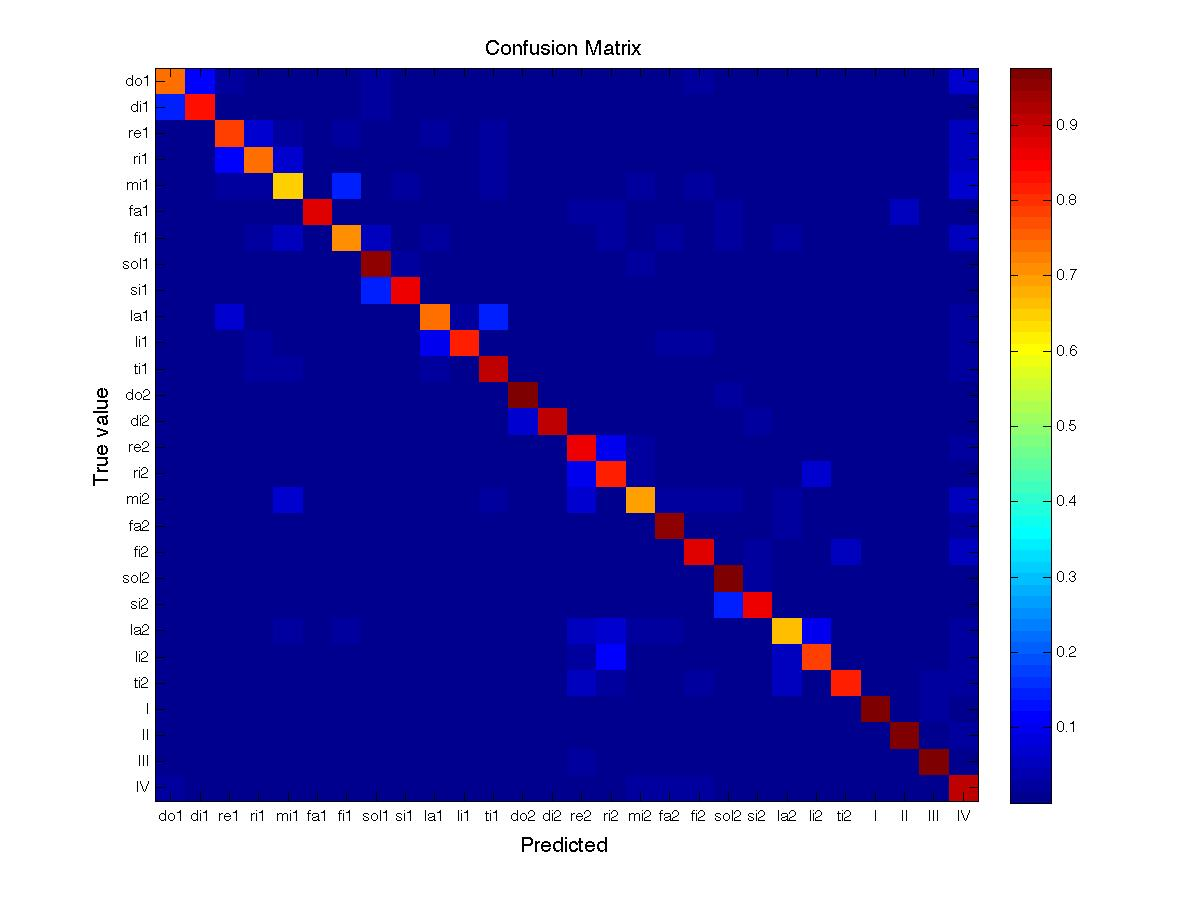
\includegraphics[width=\linewidth]{confmat/confusion.jpg}
\end{center}
\caption{confusion matrix for simple set, KNN3, per film}
\end{figure}






\subsection{Part II}

For this set of experiments the Damerau-Levenshtein distance of a sequence of generated labels to the ground truth is calculated. This value is then divided by the number of labels, 28. A low value is equal to good performance, a high value to bad. The ground truth is a list of incremented integers from 1 to 28. Since some movies are 'polluted' with incorrect hand poses and other people walking through the screen this ground truth isn't really correct. But it is very difficult to impossible to construct a good ground truth in this case, and given the fact that the goal of the recorded movies was to have people perform the 28 hand poses sequentially this is a good alternative.

simple: 0.27 average
complex: 0.35 average

ivo 0.08
hanne 0.14
gijs 0.18
ork 0.18
chu 0.19
jasberb 0.23
stratos 0.24
victoria 0.24
arjan 0.26
peter 0.26
anne 0.28
michael 0.32
gosia 0.37
koen 0.38
jasper  0.4
bas 0.44
roberto 0.47
xiaong 0.49
hamdi 0.49
sil 0.52


hanne1 9.0
hanne2 0.0
hanne3 1.0
hanne4 7.0
hanne5 2.0
ivo1 2.0
ivo2 3.0
ivo3 2.0
ivo4 3.0
ivo5 1.0
anne1 12.0
anne2 9.0
anne3 7.0
anne4 8.0
anne5 4.0
arjan1 13.0
arjan2 7.0
arjan3 7.0
arjan4 2.0
arjan5 8.0
gijs1 4.0
gijs2 5.0
gijs3 6.0
gijs4 6.0
gijs5 4.0
ork1 6.0
ork2 5.0
ork3 4.0
peter1 7.0
peter2 8.0
peter3 7.0
peter4 9.0
peter5 5.0

roberto1 19.0
roberto2 8.0
roberto3 13.0
xiaong1 17.0
xiaong2 14.0
xiaong3 10.0
jasper1 19.0
jasper2 13.0
jasper3 6.0
jasper4 6.0
jasper5 12.0
jasperb1 9.0
jasperb2 5.0
jasperb3 5.0

gosia1 16.0
gosia2 9.0
gosia3 6.0
hamdi1 14.0
hamdi2 12.0
hamdi3 15.0
michael1 6.0
michael2 8.0
michael3 13.0

sil1 14.0
sil2 17.0
sil3 13.0
koen1 11.0
koen2 9.0
koen3 11.0
bas1 15.0
bas2 12.0
bas3 9.0
chu1 8.0
chu2 6.0
chu3 2.0
stratos1 12.0
stratos2 3.0
stratos3 5.0
victoria1 9.0
victoria2 6.0
victoria3 5.0






\section{Implementation}
Sonic Gesture has been implemented in C++. Almost all computer vision algorithms used in Sonic Gesture are part of OpenCV, an open source library made for this kind of software. For the graphical interface QT is used. Sonic Gesture has been release as Open Source software and is released under the Apache license. The software can be downloaded, modified and distributed freely from:

http://code.google.com/p/sonic-gesture/

The program can capture directly from a webcam or it can read movies with recorded material. It has 2 modes, one 'finder' mode where hand poses in the video stream are detected. The second mode is the 'capture' mode, which is used to label movies. When labeling a movie in this mode a text file is created with frame positions of the labels. This can later be used to extract the correct frame and extract training data for the classifier. This mode has been used a lot during the gathering of the dataset.

\section{Time performance}
A lot of effort has been put into getting Sonic Gesture as fast as possible. Initially Sonic Gesture was written in Python and used the Python API of OpenCV. Soon it became clear that Python was to limited to do high performance graphic processing so a switch to C++ was made. 

The performance of Sonic Gesture depends on how fast the testing systems CPU power is, if the OpenCV IPP extention is used but also how fast the camera can capture frames. On a Macbook Pro, 2.4 GHz intel core 2 duo with 4 GB of memory using the build-in iSight as camera, processing one frame takes 65 ms on average. This is with the full dataset of 2072 datapoints with 3780 dimensions using the KNN classifier. KNN works fine with low numbers of datapoint, but with high numbers it starts to slow down. Still it is quite fast; around 25 ms on average. SVM will probably perform much faster with a high number of datapoints but we couldn't get the SVM implementation of OpenCV to work. An other expensive operation is the face detection algoritm, when tweaked it takes around 13 ms to locale a face in a image. Since a face position isn't required constantly this is done only every 10th frame, so valuable computation time is saved. An other surprisingly expensive operation is the resizing of a image. Resizing an image to a small size is a crucial part of the pipe line, because some operations on a big image will take too much time. But resizing a image using interpolation is a expensive operation. Where interpolation is not required, for example for rendering on the screen, it is disabled saving more computing time. 

37.9\% KNN
8.4\% color space convertion
7.6\% image resizing
2.3\% haar classifier (19% if not every 10th frame).

\section{Discussion}
As you can see there is a big difference in performance



\section{Images}

\renewcommand{\thesubfigure}{\thefigure.\roman{subfigure}}
\begin{figure}[htbp]
\begin{center}
\subfloat[Do]{\label{fig:hand_0}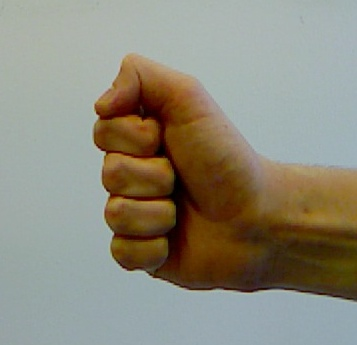
\includegraphics[width=0.2\linewidth,height=0.15\linewidth]{figures/examples/0.jpg}}
\hspace{0.03\linewidth}
\subfloat[Di]{\label{fig:hand_1}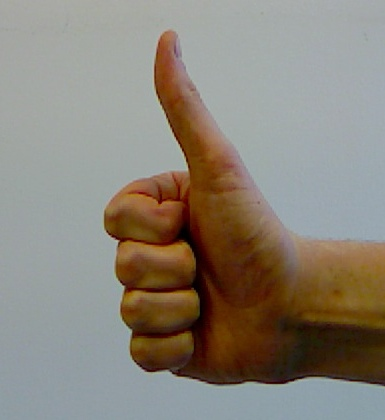
\includegraphics[width=0.2\linewidth,height=0.15\linewidth]{figures/examples/1.jpg}}
\hspace{0.03\linewidth}
\subfloat[Re]{\label{fig:hand_2}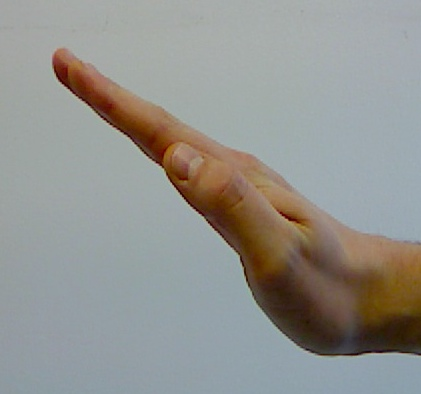
\includegraphics[width=0.2\linewidth,height=0.15\linewidth]{figures/examples/2.jpg}}
\hspace{0.03\linewidth}
\subfloat[Ri]{\label{fig:hand_3}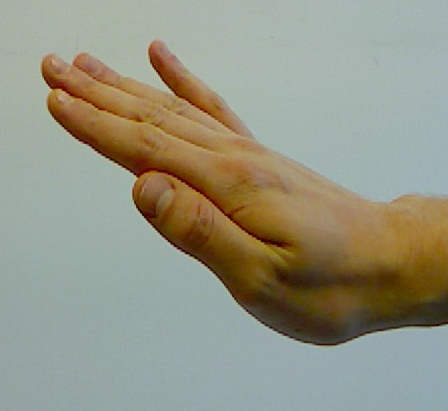
\includegraphics[width=0.2\linewidth,height=0.15\linewidth]{figures/examples/3.jpg}}
\hspace{0.03\linewidth}
\subfloat[Mi]{\label{fig:hand_4}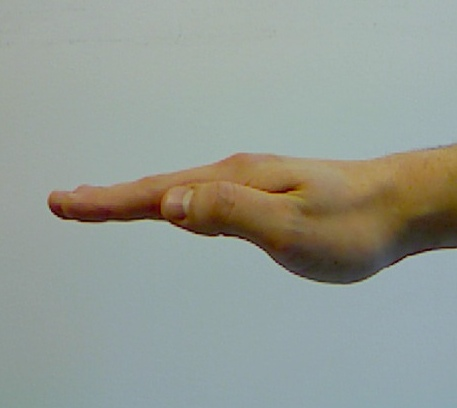
\includegraphics[width=0.2\linewidth,height=0.15\linewidth]{figures/examples/4.jpg}}
\hspace{0.03\linewidth}
\subfloat[Fa]{\label{fig:hand_5}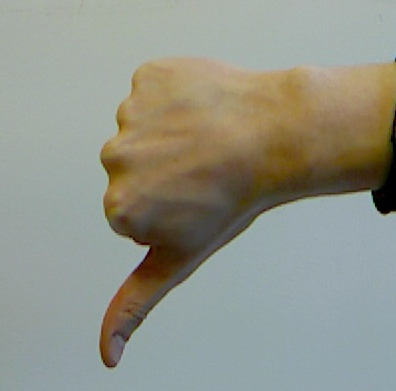
\includegraphics[width=0.2\linewidth,height=0.15\linewidth]{figures/examples/5.jpg}}
\hspace{0.03\linewidth}
\subfloat[Fi]{\label{fig:hand_6}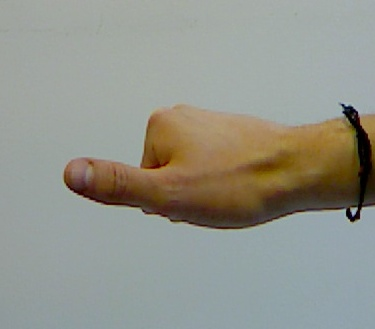
\includegraphics[width=0.2\linewidth,height=0.15\linewidth]{figures/examples/6.jpg}}
\hspace{0.03\linewidth}
\subfloat[Sol]{\label{fig:hand_7}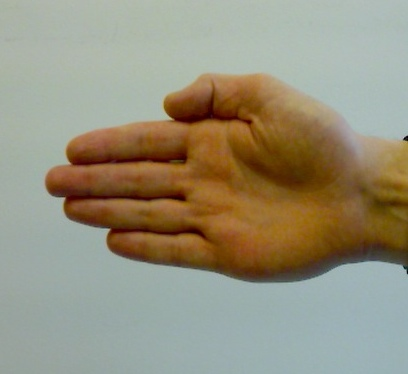
\includegraphics[width=0.2\linewidth,height=0.15\linewidth]{figures/examples/7.jpg}}
\hspace{0.03\linewidth}
\subfloat[Si]{\label{fig:hand_8}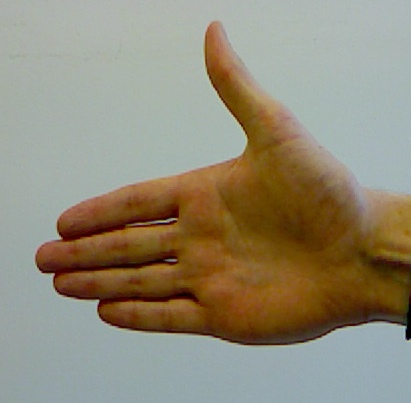
\includegraphics[width=0.2\linewidth,height=0.15\linewidth]{figures/examples/8.jpg}}
\hspace{0.03\linewidth}
\subfloat[La]{\label{fig:hand_9}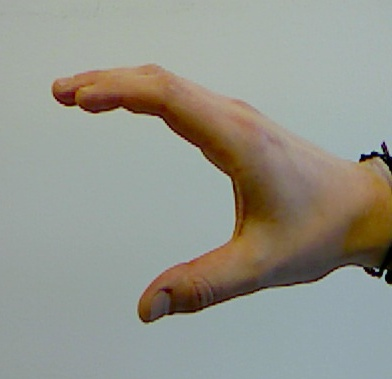
\includegraphics[width=0.2\linewidth,height=0.15\linewidth]{figures/examples/9.jpg}}
\hspace{0.03\linewidth}
\subfloat[Li]{\label{fig:hand_10}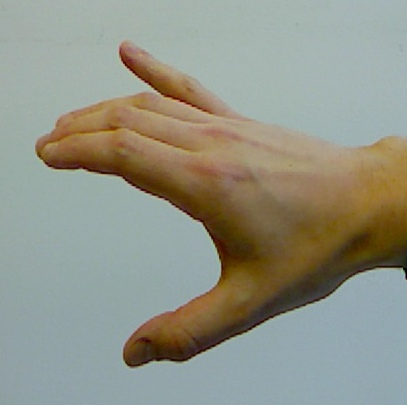
\includegraphics[width=0.2\linewidth,height=0.15\linewidth]{figures/examples/10.jpg}}
\hspace{0.03\linewidth}
\subfloat[Ti]{\label{fig:hand_11}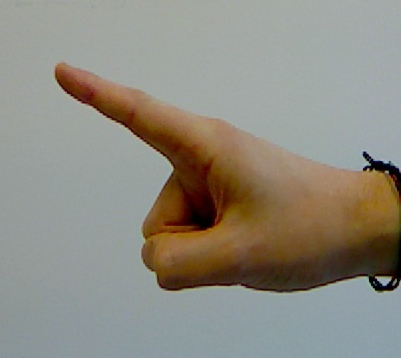
\includegraphics[width=0.2\linewidth,height=0.15\linewidth]{figures/examples/11.jpg}}
\end{center}
\caption{All mirrored Curwen hand poses}
\label{fig:hands_mirrored}
\end{figure}

\begin{figure}[htbp]
\begin{center}
\subfloat[Do]{\label{fig:hand_12}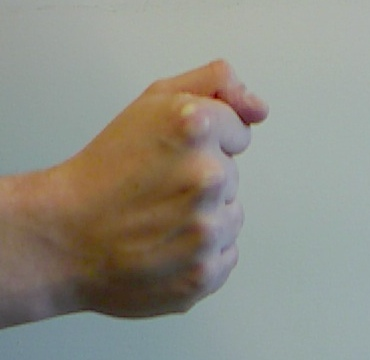
\includegraphics[width=0.2\linewidth,height=0.15\linewidth]{figures/examples/12.jpg}}
\hspace{0.03\linewidth}
\subfloat[Di]{\label{fig:hand_13}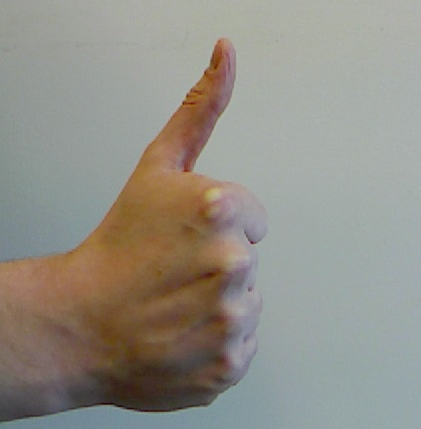
\includegraphics[width=0.2\linewidth,height=0.15\linewidth]{figures/examples/13.jpg}}
\hspace{0.03\linewidth}
\subfloat[Re]{\label{fig:hand_14}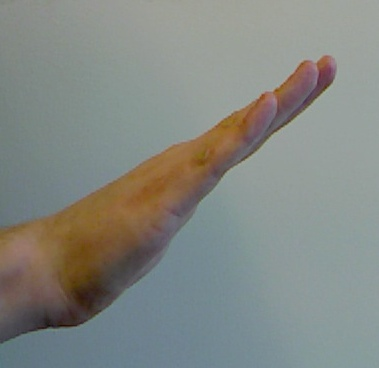
\includegraphics[width=0.2\linewidth,height=0.15\linewidth]{figures/examples/14.jpg}}
\hspace{0.03\linewidth}
\subfloat[Ri]{\label{fig:hand_15}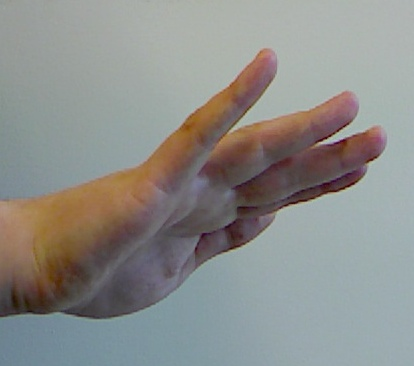
\includegraphics[width=0.2\linewidth,height=0.15\linewidth]{figures/examples/15.jpg}}
\hspace{0.03\linewidth}
\subfloat[Mi]{\label{fig:hand_16}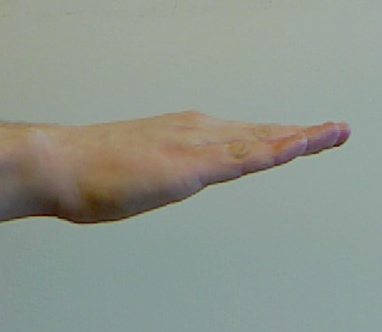
\includegraphics[width=0.2\linewidth,height=0.15\linewidth]{figures/examples/16.jpg}}
\hspace{0.03\linewidth}
\subfloat[Fa]{\label{fig:hand_17}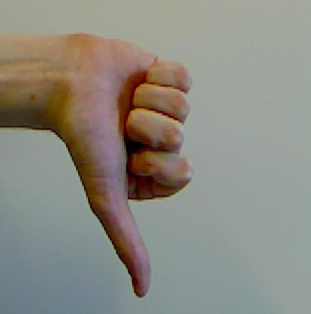
\includegraphics[width=0.2\linewidth,height=0.15\linewidth]{figures/examples/17.jpg}}
\hspace{0.03\linewidth}
\subfloat[Fi]{\label{fig:hand_18}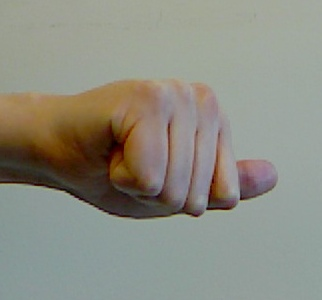
\includegraphics[width=0.2\linewidth,height=0.15\linewidth]{figures/examples/18.jpg}}
\hspace{0.03\linewidth}
\subfloat[Sol]{\label{fig:hand_19}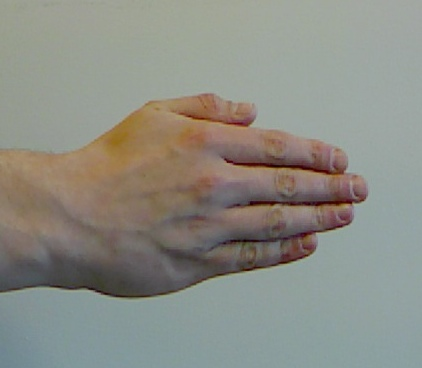
\includegraphics[width=0.2\linewidth,height=0.15\linewidth]{figures/examples/19.jpg}}
\hspace{0.03\linewidth}
\subfloat[Si]{\label{fig:hand_20}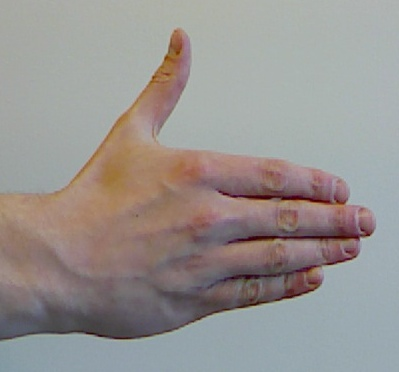
\includegraphics[width=0.2\linewidth,height=0.15\linewidth]{figures/examples/20.jpg}}
\hspace{0.03\linewidth}
\subfloat[La]{\label{fig:hand_21}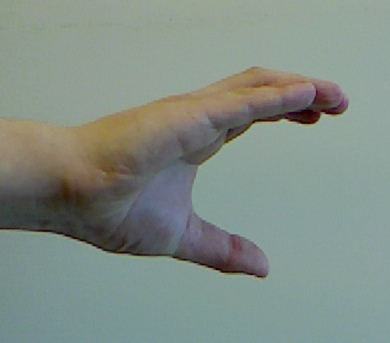
\includegraphics[width=0.2\linewidth,height=0.15\linewidth]{figures/examples/21.jpg}}
\hspace{0.03\linewidth}
\subfloat[Li]{\label{fig:hand_22}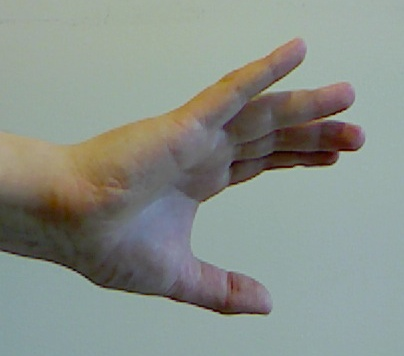
\includegraphics[width=0.2\linewidth,height=0.15\linewidth]{figures/examples/22.jpg}}
\hspace{0.03\linewidth}
\subfloat[Ti]{\label{fig:hand_23}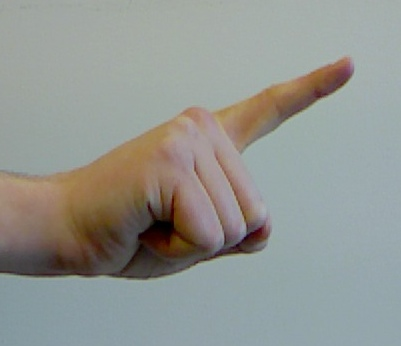
\includegraphics[width=0.2\linewidth,height=0.15\linewidth]{figures/examples/23.jpg}}
\end{center}
\caption{All Curwen hand poses}
\label{fig:hands_normal}
\end{figure}


\begin{figure}[htbp]
\begin{center}
\subfloat[Extra1]{\label{fig:hand_24}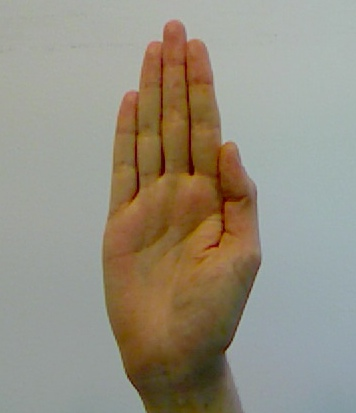
\includegraphics[width=0.2\linewidth,height=0.15\linewidth]{figures/examples/24.jpg}}
\hspace{0.03\linewidth}
\subfloat[Extra2]{\label{fig:hand_25}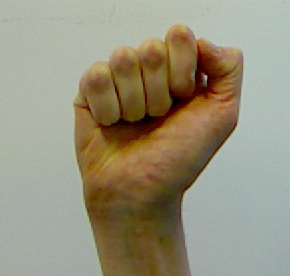
\includegraphics[width=0.2\linewidth,height=0.15\linewidth]{figures/examples/25.jpg}}
\hspace{0.03\linewidth}
\subfloat[Extra3]{\label{fig:hand_26}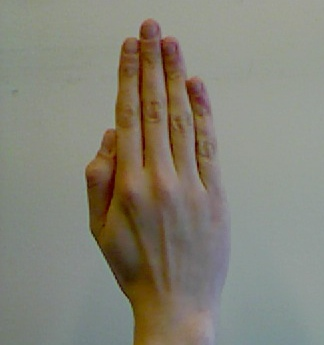
\includegraphics[width=0.2\linewidth,height=0.15\linewidth]{figures/examples/26.jpg}}
\hspace{0.03\linewidth}
\subfloat[Extra4]{\label{fig:hand_27}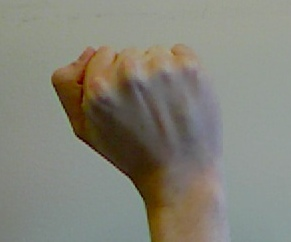
\includegraphics[width=0.2\linewidth,height=0.15\linewidth]{figures/examples/27.jpg}}
\end{center}
\caption{The extra hand poses}
\label{fig:hands_extra}
\end{figure}


\begin{figure}[htbp]
\begin{center}
\subfloat[Do]{\label{fig:gijs5_0}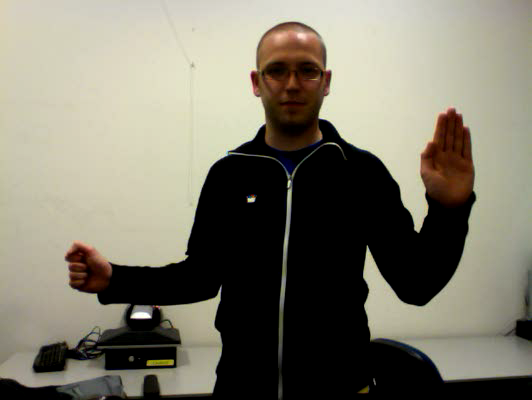
\includegraphics[width=0.2\linewidth,height=0.15\linewidth]{figures/gijs5/0.png}}
\hspace{0.03\linewidth}
\subfloat[Di]{\label{fig:gijs5_1}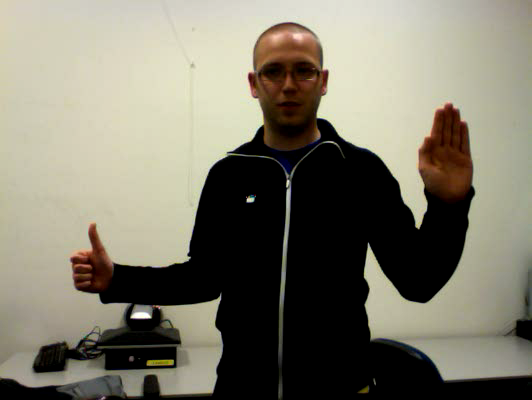
\includegraphics[width=0.2\linewidth,height=0.15\linewidth]{figures/gijs5/1.png}}
\hspace{0.03\linewidth}
\subfloat[Re]{\label{fig:gijs5_2}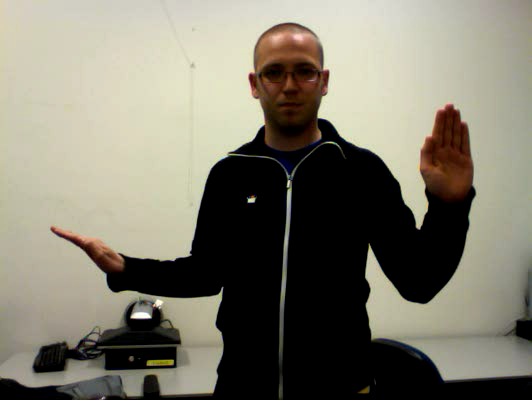
\includegraphics[width=0.2\linewidth,height=0.15\linewidth]{figures/gijs5/2.png}}
\hspace{0.03\linewidth}
\subfloat[Ri]{\label{fig:gijs5_3}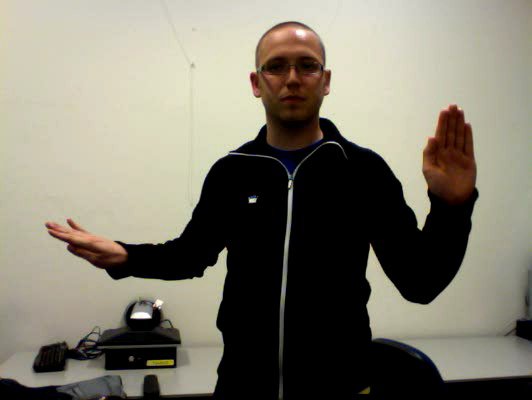
\includegraphics[width=0.2\linewidth,height=0.15\linewidth]{figures/gijs5/3.png}}
\hspace{0.03\linewidth}
\subfloat[Mi]{\label{fig:gijs5_4}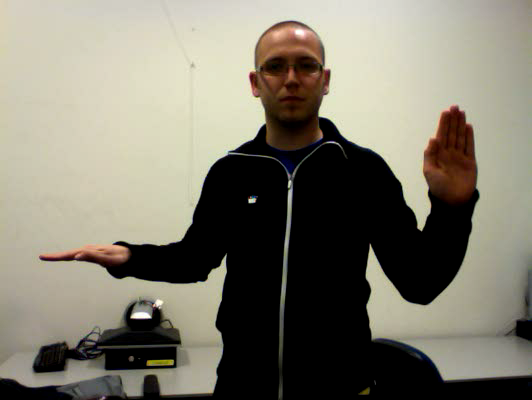
\includegraphics[width=0.2\linewidth,height=0.15\linewidth]{figures/gijs5/4.png}}
\hspace{0.03\linewidth}
\subfloat[Fa]{\label{fig:gijs5_5}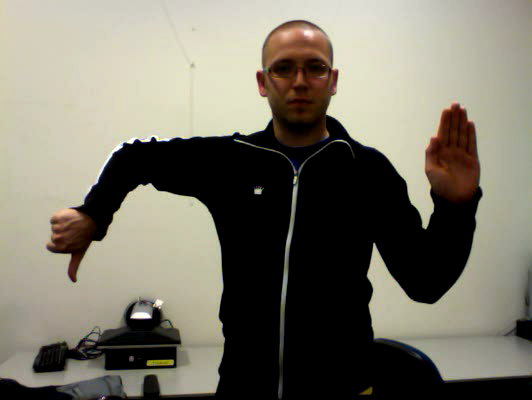
\includegraphics[width=0.2\linewidth,height=0.15\linewidth]{figures/gijs5/5.png}}
\hspace{0.03\linewidth}
\subfloat[Fi]{\label{fig:gijs5_6}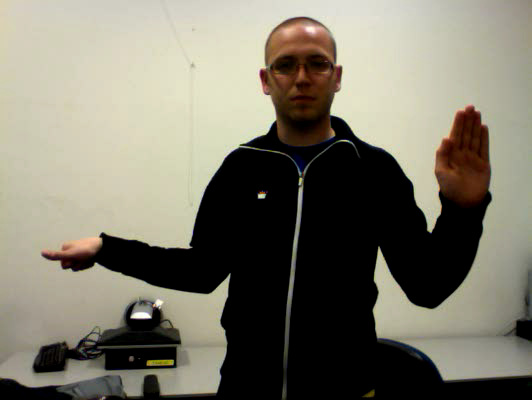
\includegraphics[width=0.2\linewidth,height=0.15\linewidth]{figures/gijs5/6.png}}
\hspace{0.03\linewidth}
\subfloat[Sol]{\label{fig:gijs5_7}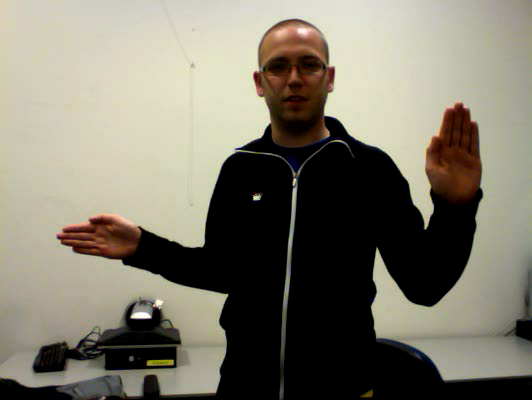
\includegraphics[width=0.2\linewidth,height=0.15\linewidth]{figures/gijs5/7.png}}
\hspace{0.03\linewidth}
\subfloat[Si]{\label{fig:gijs5_8}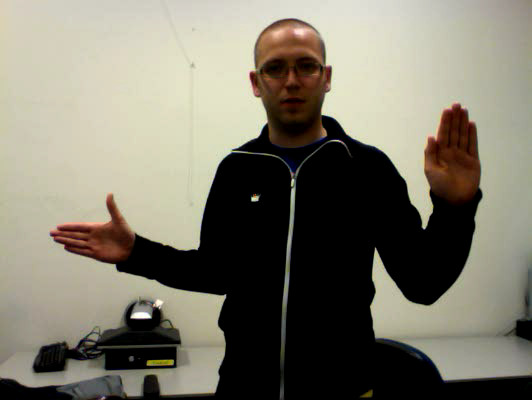
\includegraphics[width=0.2\linewidth,height=0.15\linewidth]{figures/gijs5/8.png}}
\hspace{0.03\linewidth}
\subfloat[La]{\label{fig:gijs5_9}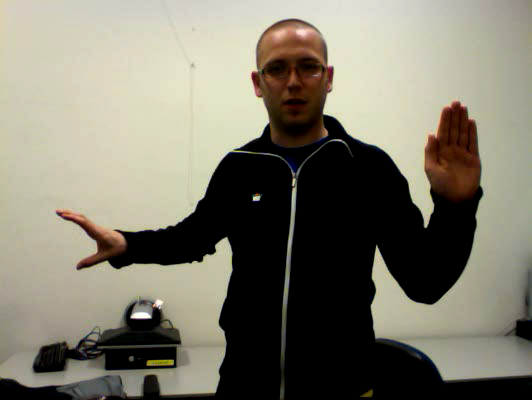
\includegraphics[width=0.2\linewidth,height=0.15\linewidth]{figures/gijs5/9.png}}
\hspace{0.03\linewidth}
\subfloat[Li]{\label{fig:gijs5_10}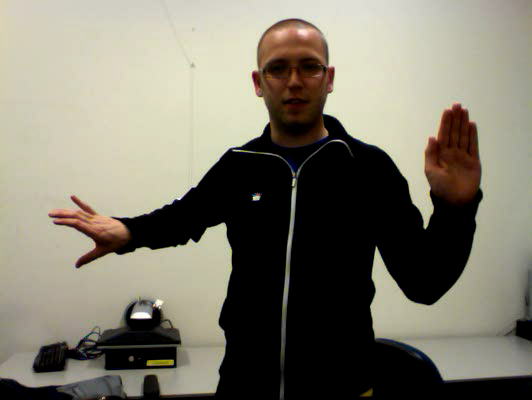
\includegraphics[width=0.2\linewidth,height=0.15\linewidth]{figures/gijs5/10.png}}
\hspace{0.03\linewidth}
\subfloat[Ti]{\label{fig:gijs5_11}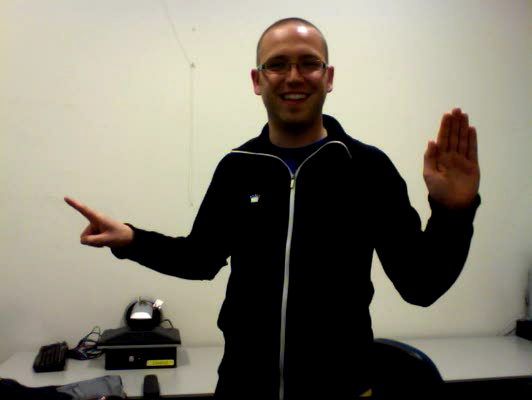
\includegraphics[width=0.2\linewidth,height=0.15\linewidth]{figures/gijs5/11.png}}
\hspace{0.03\linewidth}
\subfloat[Do]{\label{fig:gijs5_12}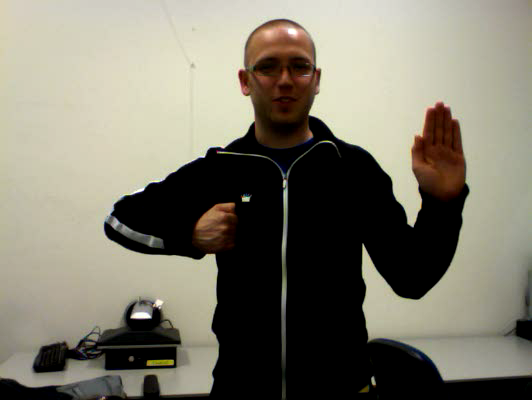
\includegraphics[width=0.2\linewidth,height=0.15\linewidth]{figures/gijs5/12.png}}
\hspace{0.03\linewidth}
\subfloat[Di]{\label{fig:gijs5_13}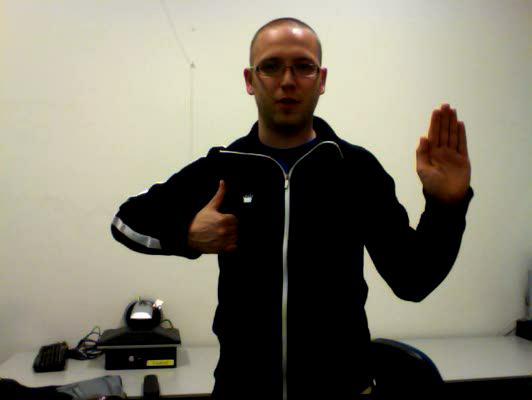
\includegraphics[width=0.2\linewidth,height=0.15\linewidth]{figures/gijs5/13.png}}
\hspace{0.03\linewidth}
\subfloat[Re]{\label{fig:gijs5_14}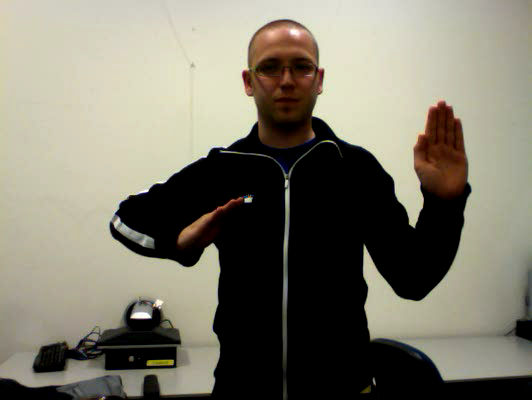
\includegraphics[width=0.2\linewidth,height=0.15\linewidth]{figures/gijs5/14.png}}
\hspace{0.03\linewidth}
\subfloat[Ri]{\label{fig:gijs5_15}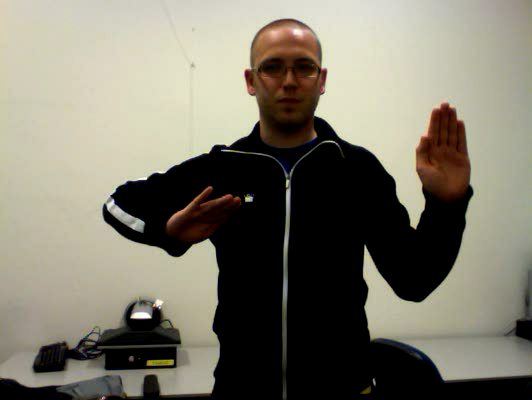
\includegraphics[width=0.2\linewidth,height=0.15\linewidth]{figures/gijs5/15.png}}
\hspace{0.03\linewidth}
\subfloat[Mi]{\label{fig:gijs5_16}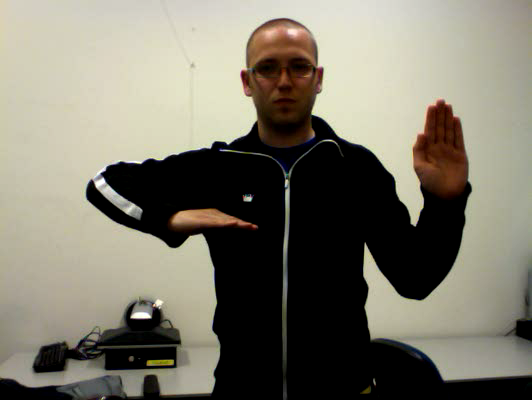
\includegraphics[width=0.2\linewidth,height=0.15\linewidth]{figures/gijs5/16.png}}
\hspace{0.03\linewidth}
\subfloat[Fa]{\label{fig:gijs5_17}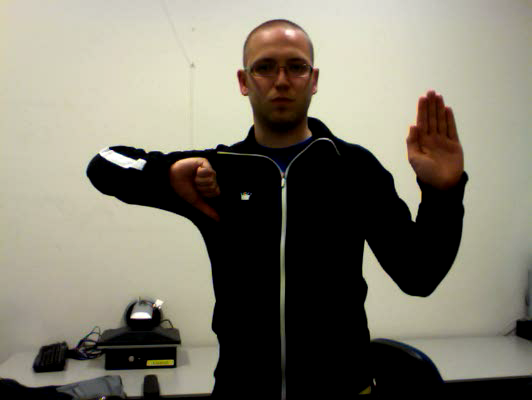
\includegraphics[width=0.2\linewidth,height=0.15\linewidth]{figures/gijs5/17.png}}
\hspace{0.03\linewidth}
\subfloat[Fi]{\label{fig:gijs5_18}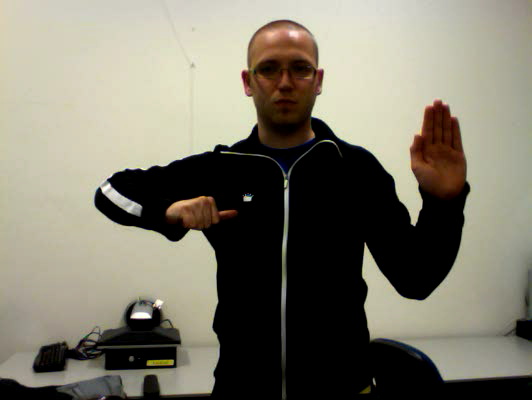
\includegraphics[width=0.2\linewidth,height=0.15\linewidth]{figures/gijs5/18.png}}
\hspace{0.03\linewidth}
\subfloat[Sol]{\label{fig:gijs5_19}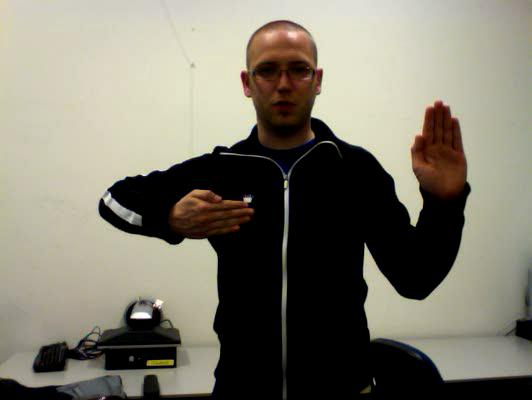
\includegraphics[width=0.2\linewidth,height=0.15\linewidth]{figures/gijs5/19.png}}
\hspace{0.03\linewidth}
\subfloat[Si]{\label{fig:gijs5_20}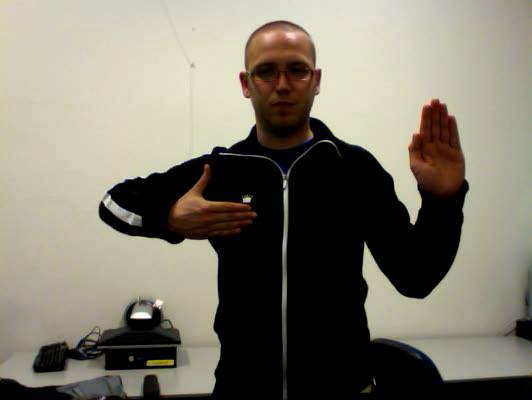
\includegraphics[width=0.2\linewidth,height=0.15\linewidth]{figures/gijs5/20.png}}
\hspace{0.03\linewidth}
\subfloat[La]{\label{fig:gijs5_21}\includegraphics[width=0.2\linewidth,height=0.15\linewidth]{figures/gijs5/21.png}}
\hspace{0.03\linewidth}
\subfloat[Li]{\label{fig:gijs5_22}\includegraphics[width=0.2\linewidth,height=0.15\linewidth]{figures/gijs5/22.png}}
\hspace{0.03\linewidth}
\subfloat[Ti]{\label{fig:gijs5_23}\includegraphics[width=0.2\linewidth,height=0.15\linewidth]{figures/gijs5/23.png}}
\hspace{0.03\linewidth}
\subfloat[Extra1]{\label{fig:gijs5_24}\includegraphics[width=0.2\linewidth,height=0.15\linewidth]{figures/gijs5/24.png}}
\hspace{0.03\linewidth}
\subfloat[Extra2]{\label{fig:gijs5_25}\includegraphics[width=0.2\linewidth,height=0.15\linewidth]{figures/gijs5/25.png}}
\hspace{0.03\linewidth}
\subfloat[Extra3]{\label{fig:gijs5_26}\includegraphics[width=0.2\linewidth,height=0.15\linewidth]{figures/gijs5/26.png}}
\hspace{0.03\linewidth}
\subfloat[Extra4]{\label{fig:gijs5_27}\includegraphics[width=0.2\linewidth,height=0.15\linewidth]{figures/gijs5/27.png}}
\end{center}
\caption{Stills from recording number 5, test subject 'gijs'}
\label{fig:gijs5}
\end{figure}



\begin{figure}[htbp]
\begin{center}
\subfloat[Do]{\label{fig:gijs5_cutout_0}\includegraphics[width=0.2\linewidth,height=0.15\linewidth]{figures/gijs5_cutout/0.jpg}}
\hspace{0.03\linewidth}
\subfloat[Di]{\label{fig:gijs5_cutout_1}\includegraphics[width=0.2\linewidth,height=0.15\linewidth]{figures/gijs5_cutout/1.jpg}}
\hspace{0.03\linewidth}
\subfloat[Re]{\label{fig:gijs5_cutout_2}\includegraphics[width=0.2\linewidth,height=0.15\linewidth]{figures/gijs5_cutout/2.jpg}}
\hspace{0.03\linewidth}
\subfloat[Ri]{\label{fig:gijs5_cutout_3}\includegraphics[width=0.2\linewidth,height=0.15\linewidth]{figures/gijs5_cutout/3.jpg}}
\hspace{0.03\linewidth}
\subfloat[Mi]{\label{fig:gijs5_cutout_4}\includegraphics[width=0.2\linewidth,height=0.15\linewidth]{figures/gijs5_cutout/4.jpg}}
\hspace{0.03\linewidth}
\subfloat[Fa]{\label{fig:gijs5_cutout_5}\includegraphics[width=0.2\linewidth,height=0.15\linewidth]{figures/gijs5_cutout/5.jpg}}
\hspace{0.03\linewidth}
\subfloat[Fi]{\label{fig:gijs5_cutout_6}\includegraphics[width=0.2\linewidth,height=0.15\linewidth]{figures/gijs5_cutout/6.jpg}}
\hspace{0.03\linewidth}
\subfloat[Sol]{\label{fig:gijs5_cutout_7}\includegraphics[width=0.2\linewidth,height=0.15\linewidth]{figures/gijs5_cutout/7.jpg}}
\hspace{0.03\linewidth}
\subfloat[Si]{\label{fig:gijs5_cutout_8}\includegraphics[width=0.2\linewidth,height=0.15\linewidth]{figures/gijs5_cutout/8.jpg}}
\hspace{0.03\linewidth}
\subfloat[La]{\label{fig:gijs5_cutout_9}\includegraphics[width=0.2\linewidth,height=0.15\linewidth]{figures/gijs5_cutout/9.jpg}}
\hspace{0.03\linewidth}
\subfloat[Li]{\label{fig:gijs5_cutout_10}\includegraphics[width=0.2\linewidth,height=0.15\linewidth]{figures/gijs5_cutout/10.jpg}}
\hspace{0.03\linewidth}
\subfloat[Ti]{\label{fig:gijs5_cutout_11}\includegraphics[width=0.2\linewidth,height=0.15\linewidth]{figures/gijs5_cutout/11.jpg}}
\hspace{0.03\linewidth}
\subfloat[Do]{\label{fig:gijs5_cutout_12}\includegraphics[width=0.2\linewidth,height=0.15\linewidth]{figures/gijs5_cutout/12.jpg}}
\hspace{0.03\linewidth}
\subfloat[Di]{\label{fig:gijs5_cutout_13}\includegraphics[width=0.2\linewidth,height=0.15\linewidth]{figures/gijs5_cutout/13.jpg}}
\hspace{0.03\linewidth}
\subfloat[Re]{\label{fig:gijs5_cutout_14}\includegraphics[width=0.2\linewidth,height=0.15\linewidth]{figures/gijs5_cutout/14.jpg}}
\hspace{0.03\linewidth}
\subfloat[Ri]{\label{fig:gijs5_cutout_15}\includegraphics[width=0.2\linewidth,height=0.15\linewidth]{figures/gijs5_cutout/15.jpg}}
\hspace{0.03\linewidth}
\subfloat[Mi]{\label{fig:gijs5_cutout_16}\includegraphics[width=0.2\linewidth,height=0.15\linewidth]{figures/gijs5_cutout/16.jpg}}
\hspace{0.03\linewidth}
\subfloat[Fa]{\label{fig:gijs5_cutout_17}\includegraphics[width=0.2\linewidth,height=0.15\linewidth]{figures/gijs5_cutout/17.jpg}}
\hspace{0.03\linewidth}
\subfloat[Fi]{\label{fig:gijs5_cutout_18}\includegraphics[width=0.2\linewidth,height=0.15\linewidth]{figures/gijs5_cutout/18.jpg}}
\hspace{0.03\linewidth}
\subfloat[Sol]{\label{fig:gijs5_cutout_19}\includegraphics[width=0.2\linewidth,height=0.15\linewidth]{figures/gijs5_cutout/19.jpg}}
\hspace{0.03\linewidth}
\subfloat[Si]{\label{fig:gijs5_cutout_20}\includegraphics[width=0.2\linewidth,height=0.15\linewidth]{figures/gijs5_cutout/20.jpg}}
\hspace{0.03\linewidth}
\subfloat[La]{\label{fig:gijs5_cutout_21}\includegraphics[width=0.2\linewidth,height=0.15\linewidth]{figures/gijs5_cutout/21.jpg}}
\hspace{0.03\linewidth}
\subfloat[Li]{\label{fig:gijs5_cutout_22}\includegraphics[width=0.2\linewidth,height=0.15\linewidth]{figures/gijs5_cutout/22.jpg}}
\hspace{0.03\linewidth}
\subfloat[Ti]{\label{fig:gijs5_cutout_23}\includegraphics[width=0.2\linewidth,height=0.15\linewidth]{figures/gijs5_cutout/23.jpg}}
\hspace{0.03\linewidth}
\subfloat[Extra1]{\label{fig:gijs5_cutout_24}\includegraphics[width=0.2\linewidth,height=0.15\linewidth]{figures/gijs5_cutout/24.jpg}}
\hspace{0.03\linewidth}
\subfloat[Extra2]{\label{fig:gijs5_cutout_25}\includegraphics[width=0.2\linewidth,height=0.15\linewidth]{figures/gijs5_cutout/25.jpg}}
\hspace{0.03\linewidth}
\subfloat[Extra3]{\label{fig:gijs5_cutout_26}\includegraphics[width=0.2\linewidth,height=0.15\linewidth]{figures/gijs5_cutout/26.jpg}}
\hspace{0.03\linewidth}
\subfloat[Extra4]{\label{fig:gijs5_cutout_27}\includegraphics[width=0.2\linewidth,height=0.15\linewidth]{figures/gijs5_cutout/27.jpg}}
\end{center}
\caption{Cutout hands, test subject 'gijs' recording number 5}
\label{fig:gijs5_cutout}
\end{figure}



